

\section{Введение}


\subsection{Цель работы}

Цель данной лабораторной работы заключается в изучении методов многократных прямых измерений физических величин, а также в освоении процедур обработки полученных данных для повышения их точности и достоверности. Для достижения поставленной цели необходимо выполнить серию измерений одной и той же физической величины, обработать полученные результаты с помощью статистических методов и оценить погрешности измерений.

Методы исследования включают использование стандартных измерительных приборов, математическое моделирование процессов, а также статистическую обработку данных с применением соответствующих формул для оценки погрешностей и анализа результатов.


\subsection{Решаемые задачи}
\begin{enumerate}
  \item Освоение методики использования измерительного прибора для
многократного прямого измерения физической величины.
  \item Выполнение простейшей статистической обработки серии
результатов наблюдений при прямых измерениях.
\end{enumerate}

\section{Основная часть}

\subsection{Теоретическая часть}

В данной лабораторной работе используется метод многократных прямых измерений для регистрации данных с частотомера, который отображает временные диапазоны регистрации сигналов с генератора. Мы проводим серию измерений с целью определения средней величины, отклонений и оценки погрешностей, связанных с приборами.

Формула для нахождения среднего арифметического $\overline{f}$:
\begin{equation}
  \overline{f} = \frac{\sum_{i=1}^{n} f_i}{n}
\end{equation}
где $n$ - количество результатов отдельных наблюдений, $f_i$ - результат измерения отдельного наблюдения.

Вычисление погрешности прибора $\Delta f_{\text{приб}}$ определяется следующей формулой:
\begin{equation}
  \delta f = \pm ( \gamma_0 +  \frac{f_{\text{0}}}{f_{\text{х}}*10^n})* 100\%
\end{equation}
Среднеквадратичное отклонение $\sigma$:
\begin{equation}
  \sigma \approx \sqrt{\frac{1}{n-1} \sum_{i = 1}^{n} (f_i -\overline{f}^2)}
\end{equation}
Средняя квадратичная погрешность среднего $\Delta f$:
\begin{equation}
  \Delta f = \sigma_{\overline{f}} \approx \frac{\sigma}{\sqrt{n}}
\end{equation}

\subsection{Эксперимент}
От генератора сигналов на частотомер подается последовательность
прямоугольных импульсов, диапозоны которых были заданы $0-10^5$ кГц для грубой шкалы и $0-10^4$ кГц для точной шкалы.
Частота следования импульсов многократно измерялась с помощью частотомера на двух
шкалах: грубой и точной. В качестве генератора импульсов использовался
генератор Г5-2А, а в качестве частотомера – Ч3—32. Все данные в ходе эксперимента записывались в протокол наблюдения. \\

\begin{figure}[H]
\centering
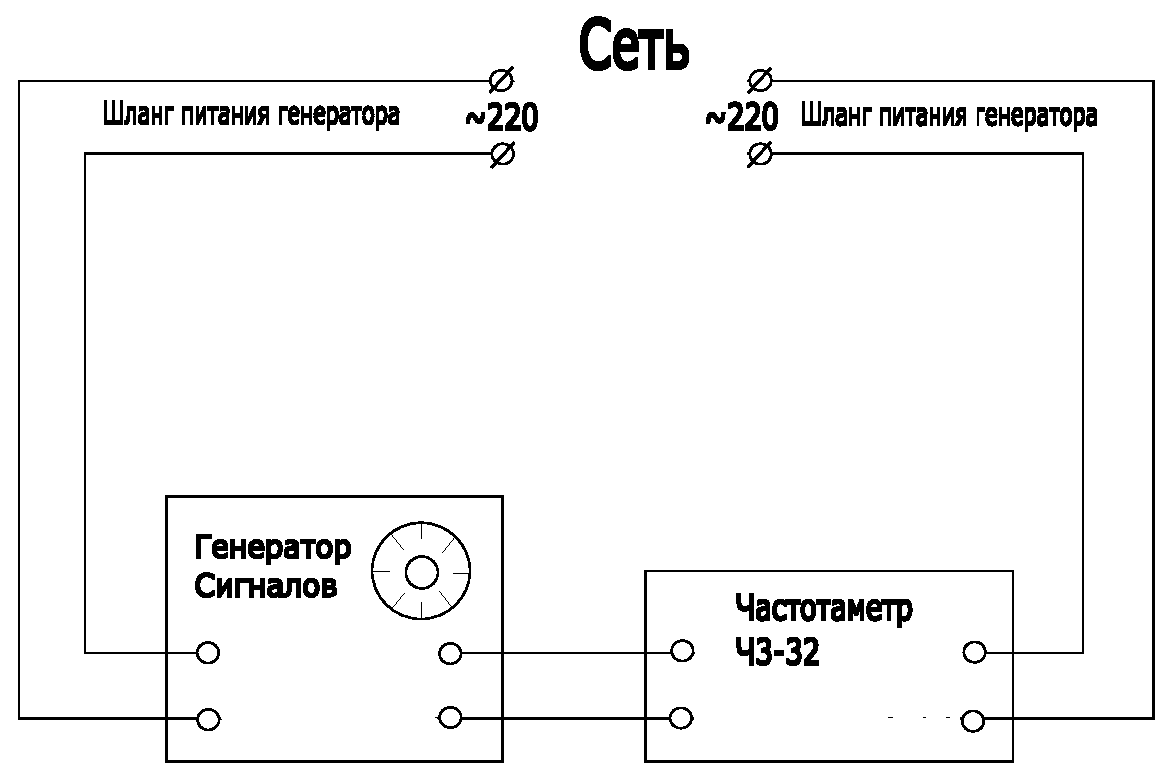
\includegraphics[width=0.6\textwidth]{sketch1.eps}
\caption{Схема установки}
\label{fig:sketch}
\end{figure}

\begin{figure}[H]
\centering
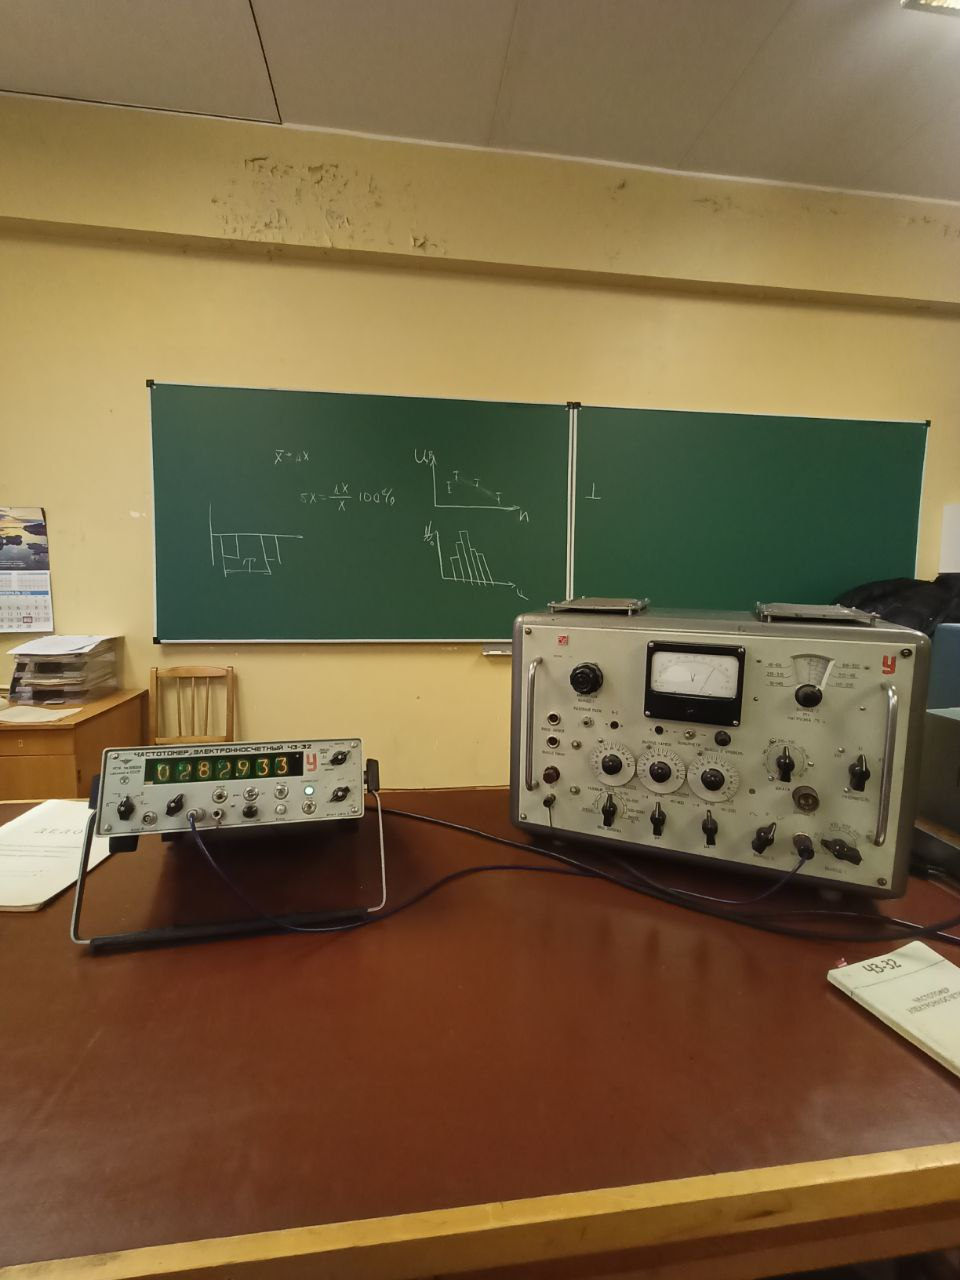
\includegraphics[width=0.6\textwidth]{Device.png}
\caption{Фотография установки}
\label{fig:device}
\end{figure}


\subsection{Обработка данных и обсуждение результатов}
Для написания программы, вычисляющей все требуемые данные, используется язык C++; среда разработки - Visual Studio.
Код полностью расположен в репозитории на GitHub.


\subsubsection{Исходный код} 

Программа выполняет обработку данных, считанных из файлов с точными и грубыми измерениями. Вначале открывается файл с точными значениями, и все строки с числами считываются в вектор. После этого вычисляется среднее значение для этих данных, и это значение используется для вычисления отклонений от среднего для каждого числа в векторе. Далее программа рассчитывает квадрат этих отклонений, что соответствует стандартному отклонению, и выводит результаты.

После вычисления стандартного отклонения программа вычисляет среднюю погрешность прибора, используя заранее определённые параметры. Далее, с использованием функции, которая рассчитывает погрешности на основе значений времени и других параметров, программа выводит погрешности для каждого значения.

Аналогично проводятся измерения и для грубых, и для точных значений.

\begin{lstlisting}[label=listing1, caption=Вычисление среднего,]
/ Функции для вычислений
double avarage(const vector<double>& data)
{
    double sum = 0.0;
    for (double u : data)
    {
        sum += u;
    }
    return sum / data.size();
}

vector<double> standartDeviation(vector<double>& randDevAr)
{
    vector<double> standAr;
    for (int i = 0; i < randDevAr.size(); i++)
    {
        double t = randDevAr[i];
        standAr.push_back(t * t);
    }
    return standAr;
}

vector<double> randomDeviation(const vector<double>& data, double avarage)
{
    vector<double> randDevAr;
    for (int i = 0; i < data.size(); i++)
    {
        randDevAr.push_back(data[i] - avarage);
    }

    return randDevAr;
}

vector<double> calculateDeltaf(const vector<double>& fx_values, double gamma0, double f0, double f_avg)
{
    vector<double> deltaf_results;
    for (double fx : fx_values)
    {
        double gamma_f = gamma0 + (f0 / fx);
        deltaf_results.push_back(gamma_f * f_avg);
    }
    return deltaf_results;
}


    // Вычисление среднего значения
    double mean = avarage(values);
    cout << "Среднее значение (точные): " << mean << endl;

    // Вычисление отклонений от среднего для каждого значения
    cout << "Отклонения от среднего: " << endl;

    vector<double> ar1 = randomDeviation(values, mean);

    for (int i = 0; i < ar1.size(); i++)
    {
        cout << ar1[i] << "\n";
    }
    cout << endl;

    // Вычисление стандартного отклонения

    cout << "Стандартное отклонение: " << endl;

    vector<double> ar2 = standartDeviation(ar1);
    for (int i = 0; i < ar2.size(); i++)
    {
        cout << ar2[i] << "\n";
    }
    cout << endl;

    // Вычисление средней погрешности прибора
    cout << "Средняя погрешность прибора: " << endl;

    cout << (gamma0 + (f0 / mean)) * mean << "\n";
    cout << endl;

    // Вычисление погрешностей
    cout << "Погрешности (точные): " << endl;

    vector<double> delta_f1 = calculateDeltaf(values, gamma0, f0, mean);
    for (int i = 0; i < delta_f1.size(); i++)
    {
        cout << delta_f1[i] << "\n";
    }
    cout << endl;
}

\end{lstlisting}

\clearpage
\subsubsection{Таблицы}
\begin{center}
\begin{table}[h!]
\centering
\caption{Результаты грубых измерений}
\label{tabl:1}
\begin{tabular}{|c|c|c|c|c|}
\hline
\begin{minipage}{7mm}
    № п.п. 
\end{minipage}&
\begin{minipage}{5cm}
    Диапазон показаний использованной шкалы прибора
\end{minipage} &
\begin{minipage}{5cm}
    Результаты отдельных наблюдений ($f_i$)
\end{minipage} &
\begin{minipage}{5cm}
    Погрешность прибора на данной шкале ($\Delta f_{\text{приб}}$)
\end{minipage}\\
\hline
{}&кГц&кГц&кГц\\
\hline
1 &	$0-10^5$ &	4,52 & 0.01 \\
2 &	$0-10^5$ &	4,52 & 0.01 \\
3 &	$0-10^5$ &	4,54 & 0.01 \\
4 &	$0-10^5$ &	4,52 & 0.01 \\
5 & $0-10^5$ &	4,50 & 0.01 \\
6 & $0-10^5$ &	4,52 & 0.01 \\
7 & $0-10^5$ &	4,52 & 0.01 \\
8 & $0-10^5$ &	4,52 & 0.01 \\
9 & $0-10^5$ &	4,50 & 0.01 \\
10& $0-10^5$ &	4,52 & 0.01 \\
\hline
\end{tabular}
\end{table}
\end{center}

\begin{center}
\begin{table}[h!]
\centering
\caption{Результаты точных измерений}
\label{tabl:2}
\begin{tabular}{|c|c|c|c|}
\hline
\begin{minipage}{7mm}
    № п.п. 
\end{minipage}&
\begin{minipage}{5cm}
    Результаты отдельных наблюдений ($f_i$)
\end{minipage} &
\begin{minipage}{5cm}
    Случайные отклонения от среднего $d_i = f_i - \overline{f}$
\end{minipage} &
\begin{minipage}{5cm}
     $d_i^2 = (f_i - \overline{f})^2$
\end{minipage}\\
\hline
{}&кГц&кГц&кГц\\
\hline
1 & 4,524 & 0,002 & $2,496*10^{-7}$ \\
2 & 4,514 & -0,008 & $7,090*10^{-6}$ \\
3 & 4,509 & -0,013 & $1,801*10^{-5}$ \\
4 & 4,514 & -0,008 & $7,090*10^{-6}$ \\
5 & 4,512 & -0,010 & $1,086*10^{-5}$ \\
6 & 4,504 & -0,018 & $3,393*10^{-5}$ \\
7 & 4,496 & -0,026 & $6,980*10^{-5}$ \\
8 & 4,490 & -0,032 & $1,051*10^{-4}$ \\
9 & 4,498 & -0,024 & $5,963*10^{-5}$ \\
10 & 4,497 & -0,025 & $6,462*10^{-5}$ \\
11 & 4,491 & -0,031 & $9,872*10^{-5}$ \\
12 & 4,508 & -0,014 & $2,079*10^{-5}$ \\
13 & 4,502 & -0,020 & $4,170*10^{-5}$ \\
14 & 4,530 & 0,008 & $5,746*10^{-6}$ \\
15 & 4,538 & 0,016 & $2,427*10^{-5}$ \\
\hline
\end{tabular}
\end{table}
\end{center}

\begin{center}
\begin{table}[h!]
\centering
\caption{Результаты точных измерений}
\label{tabl:2}
\begin{tabular}{|c|c|c|c|c|}
\hline
\begin{minipage}{7mm}
    № п.п. 
\end{minipage}&
\begin{minipage}{5cm}
    Результаты отдельных наблюдений (fi)
\end{minipage} &
\begin{minipage}{5cm}
    Случайные отклонения от среднего $d_i = f_i - \overline{f}$
\end{minipage} &
\begin{minipage}{5cm}
     $d_i^2 = (f_i - \overline{f})^2$
\end{minipage}\\
\hline
{}&кГц&кГц&кГц\\
\hline
16 & 4,548 & 0,026 & $6,543*10^{-5}$ \\
17 & 4,544 & 0,022 & $4,657*10^{-5}$ \\
18 & 4,542 & 0,020 & $3,834*10^{-5}$ \\
19 & 4,532 & 0,010 & $9,178*10^{-6}$ \\
20 & 4,528 & 0,006 & $3,114*10^{-6}$ \\
21 & 4,526 & 0,004 & $1,282*10^{-6}$ \\
22 & 4,520 & -0,002 & $5,856*10^{-7}$ \\
23 & 4,512 & -0,010 & $1,086*10^{-5}$ \\
24 & 4,516 & -0,006 & $4,122*10^{-6}$ \\
25 & 4,524 & 0,002 & $2,496*10^{-7}$ \\
26 & 4,518 & -0,004 & $1,954*10^{-6}$ \\
27 & 4,520 & -0,002 & $5,856*10^{-7}$ \\
28 & 4,514 & -0,008 & $7,090*10^{-6}$ \\
29 & 4,516 & -0,006 & $4,122*10^{-6}$ \\
30 & 4,514 & -0,008 & $7,090*10^{-6}$ \\
31 & 4,524 & 0,002 & $2,496*10^{-7}$ \\
32 & 4,536 & 0,014 & $1,844*10^{-5}$ \\
33 & 4,540 & 0,018 & $3,091*10^{-5}$ \\
34 & 4,532 & 0,010 & $9,178*10^{-6}$ \\
35 & 4,538 & 0,016 & $2,427*10^{-5}$ \\
36 & 4,538 & 0,016 & $2,427*10^{-5}$ \\
37 & 4,530 & 0,008 & $5,746*10^{-6}$ \\
38 & 4,536 & 0,014 & $1,844*10^{-5}$ \\
39 & 4,530 & 0,008 & $5,746*10^{-6}$ \\
40 & 4,524 & 0,002 & $2,496*10^{-7}$ \\
41 & 4,522 & -0,001 & $1,764*10^{-8}$ \\
42 & 4,524 & 0,002 & $2,496*10^{-7}$ \\
43 & 4,534 & 0,012 & $1,341*10^{-4}$ \\
44 & 4,534 & 0,012 & $1,341*10^{-4}$ \\
45 & 4,534 & 0,012 & $1,341*10^{-4}$ \\
46 & 4,530 & 0,008 & $5,746*10^{-6}$ \\
47 & 4,530 & 0,008 & $5,746*10^{-6}$ \\
48 & 4,530 & 0,008 & $5,746*10^{-6}$ \\
49 & 4,528 & 0,006 & $3,114*10^{-6}$ \\
50 & 4,526 & 0,004 & $1,282*10^{-6}$ \\
\hline
\end{tabular}
\end{table}
\end{center}

\begin{table}[h!]
\centering
\caption{Таблица для построения гистограммы и кривой распределения}
\label{tabl:1}
\begin{tabular}{|c|c|c|c|c|}
\hline
\begin{minipage}{7mm}
    № интервала 
\end{minipage}&
\begin{minipage}{5cm}
    Границы интервалов (ширина интервала $\Delta h = 0.01$)
\end{minipage} & 
\begin{minipage}{5cm}
    Число случаев ($\Delta n$), когда результат наблюдения попадает в данный интервал
\end{minipage} & 
\begin{minipage}{5cm}
    Доля (часть) полного числа результатов, попадающих в данный интервал ($\delta n = \frac{\Delta n}{n}$)
\end{minipage}\\
\hline
1 & 4.490 - 4.500 & 5 & 0.083 \\
2 & 4.500 - 4.510 & 6 & 0.100 \\
3 & 4.510 - 4.520 & 9 & 0.150 \\
4 & 4.520 - 4.530 & 19 & 0.317 \\
5 & 4.530 - 4.540 & 16 & 0.267 \\
6 & 4.540 - 4.550 & 5 & 0.083 \\
\hline
\end{tabular}
\end{table}

\subsubsection{Графики}


\begin{figure}[ht!]
\centering
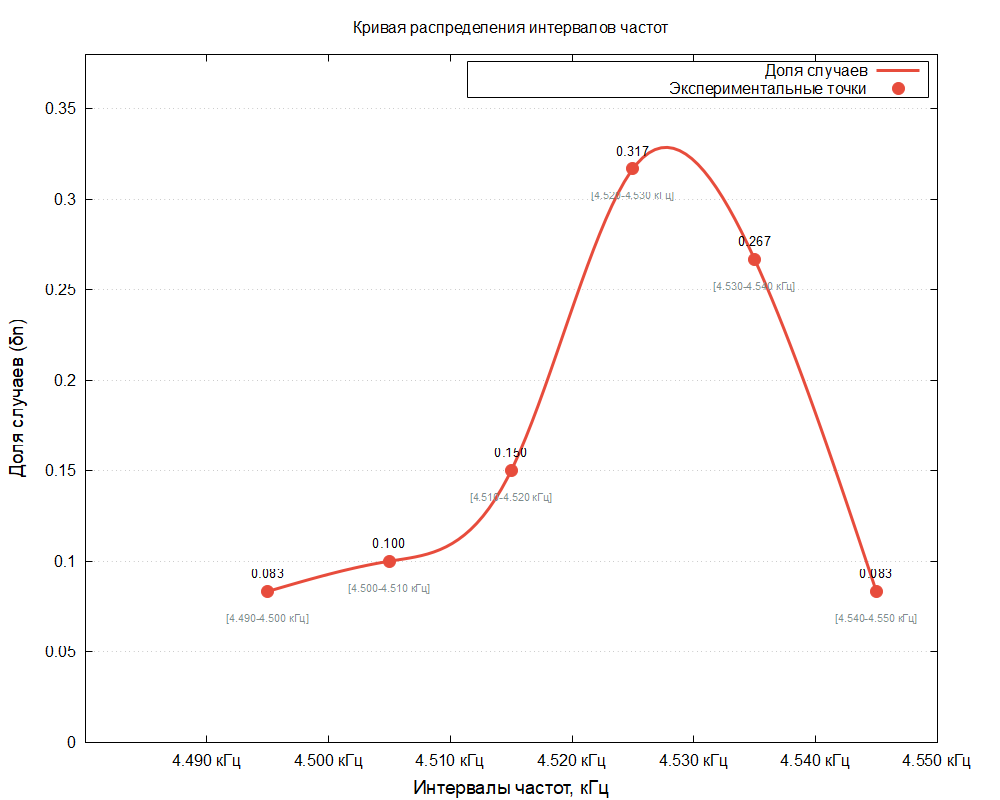
\includegraphics[width=0.8\textwidth]{smooth_distribution_ms.png}
\caption{Плотность распределения}
\label{fig:plot}
\end{figure}

\begin{figure}[ht!]
\centering
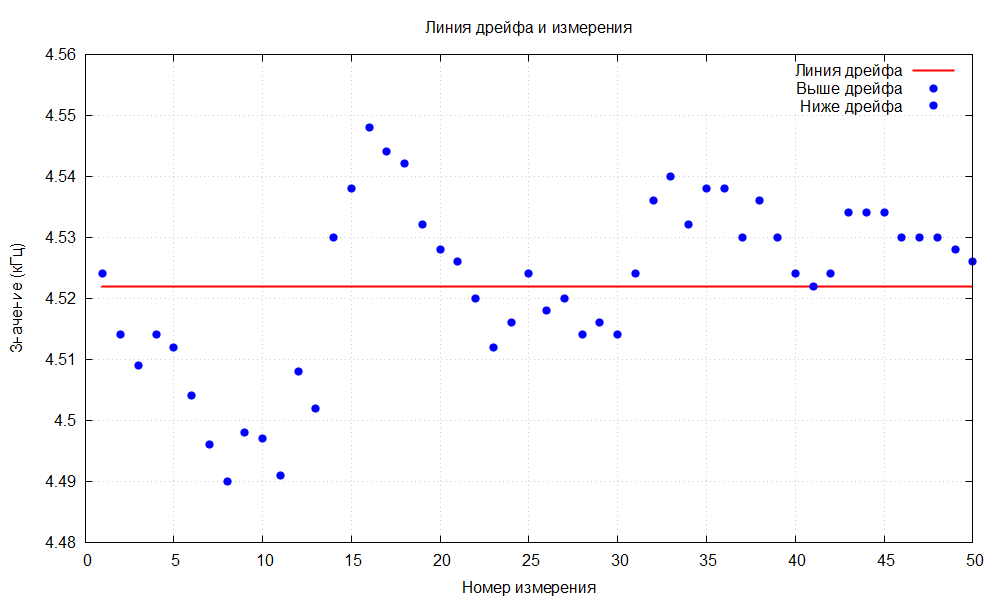
\includegraphics[width=0.8\textwidth]{plot2_drift.png}
\caption{Зависимость измерений от времени}
\label{fig:plot}
\end{figure}

\begin{figure}[ht!]
\centering
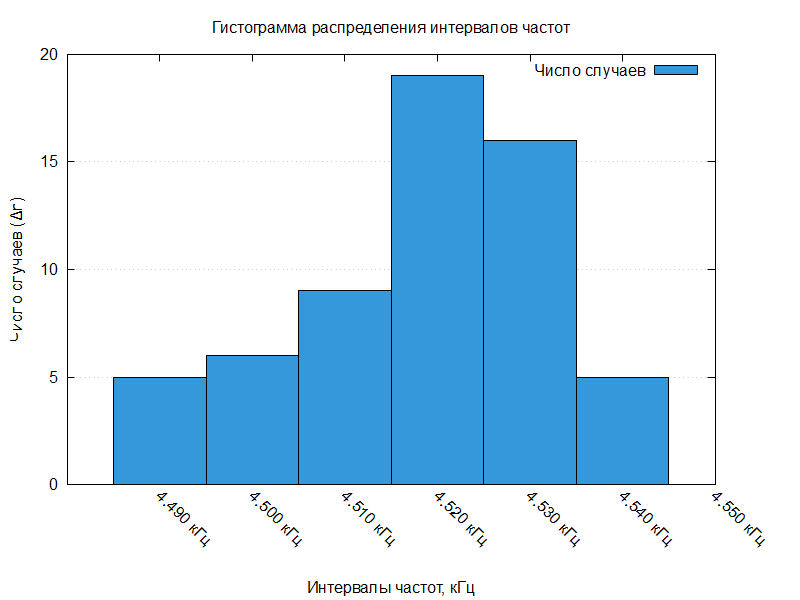
\includegraphics[width=0.8\textwidth]{histogram_ms.png}
\caption{Гистограмма}
\label{fig:plot}
\end{figure}

\clearpage

Среднеквадратичное отклонение:
\begin{equation}
    \sigma \approx \sqrt{\frac{\sum_{i=1}^{n}(f_i-\overline{f})^{2}}{n-1}}=1,405*10^{-2}
\end{equation} 
Дисперсия:
\begin{equation}
    \sigma^2=1,975\cdot10^{-4}
\end{equation}
Средняя квадратичная погрешность среднего:
\begin{equation}
    \Delta f \approx \frac{\sigma}{\sqrt{n}}=1,987 \cdot 10^{-3} \text{ кГц}
\end{equation}
 Погрешнность прибора на грубой шкале:
\begin{equation}
    \Delta f_\text{приб} = \pm 0.01  \text{ кГц}
\end{equation}
Погрешность прибора на точной шкале:
\begin{equation}
    \Delta f_\text{приб} = \pm 0.001  \text{ кГц}
\end{equation}
Ищем суммарнаую погрешность (случай одинакового порядка средней квадра-
тичной погрешности и погрешности прибора):\\
Максимальное значение суммарной погрешности:
\begin{equation}
	\Delta f_\text{сум}^{\text{макс}} = 3 \cdot \Delta f + \Delta f_\text{приб} = 3 \cdot 1.987\cdot10^{-3} + 0.001 = 0.007 \text{ кГц}
\end{equation}
Минимальное значение суммарной погрешности:
\begin{equation}
	\Delta f_\text{сум}^{\text{мин}} = \sqrt{(\frac{\Delta f_\text{приб}}{3})^2+\Delta f ^2} = 0.002 \text{ кГц}
\end{equation}

Окончательный результат:
\begin{equation}
    f=f_\text{ср}\pm\Delta f_\text{сум}^{\text{макс}} = 4.522 \pm 0.007 \text{ кГц}
\end{equation}

\clearpage
\section{Выводы}
В ходе выполнения лабораторной работы были достигнуты поставленные цели по изучению методов многократных прямых измерений физических величин и освоению процедур статистической обработки экспериментальных данных.

Экспериментальная часть исследования включала сбор и систематизацию данных, их визуализацию в виде таблиц, гистограмм и диаграмм с использованием специализированного программного обеспечения.

Непосредственная работа с лабораторными установками значительно углубила понимание изучаемых процессов, обеспечив наглядность и практическую подтверждаемость теоретических положений. 

Полученные навыки работы с измерительными приборами и обработки экспериментальных данных имеют важное значение для дальнейшей научно-исследовательской деятельности.
% Список литературы
% Для отчёта он не обязателен
\begin{thebibliography}{9}

%ссылка на репозиторий с исходныим кодом отчета и всех расчетных программ обязательна 
\bibitem{repo}
\url{https://github.com/st117168/2025-4sem-Measurement_methods/tree/main/Workshop1} 

\end{thebibliography}


